\section{Approach}
\label{sec:approach}
In this section, we have proposed a comprehensive approach to address the discussed problem. 
%In our approach, at first we have proposed a validation technique and utilized that to achieve accountability of a DNN model.
In the \S\ref{sec:background}, we have discussed the forward and backward propagation. In the two-step learning process, random initialization plays a crucial role in model validation. 
%In Figure \ref{fig:rq5}, a traditional DNN model iteratively chooses the input. The choice can be a single input at a time or a group of inputs. Three known parameters require random initialization i.e., seed, weight, and bias \cite{sutskever2013importance}. 
%Our hypothesis in this study states that \emph{$H_0$: Knowing the distribution of the random initialized parameter can provide the distribution of the output parameter, e.g., accuracy metric.} Based on this hypothesis, we select the operations that require random initialization. Then, with the known distribution, we perform the model operations as follows.
In Figure \ref{fig:flow}, we have depicted the overview of the proposed approach. We begin our approach by mining the documentation of \emph{Keras} DNN library and manually identify the parameters responsible for the randomly initialization. Thereupon, we compute the optimized value for those parameters using an adaptive simulated annealing algorithm. The aforementioned process produces a near optimum value for the output metric. At last, we made a user-intent based accountable DNN accuracy search that restricts a model so that near optimal accuracy can be achieved in terms of time, trial, and gain constraints.
%\begin{equation}
%f(\sum_{\chi}{W_iX_i+B}), \chi\sim D(\mu, \sigma^2)
%\end{equation}
%In the equation above, the traditional dense operation has been depicted as an example, where, $W_i$, $X_i$, $B_i$, $f()$, and $D$ represents the weight, input, bias, the activation function, and a unknown distribution of the operations respectively that require random initialization. The output of this learning process will be an interval of value rather than a single concrete value. In Figure \ref{fig:rq5}, we have depicted a similar scenario that includes the learning of the distribution, which results in an interval reported as "[Low, High]". The interval is similar to any algorithmic evaluation with the best-case and worst-case scenario. 
%In the diagram \fignref{fig:flow}, 
Our methodology has been discussed as follows.
\begin{figure}
	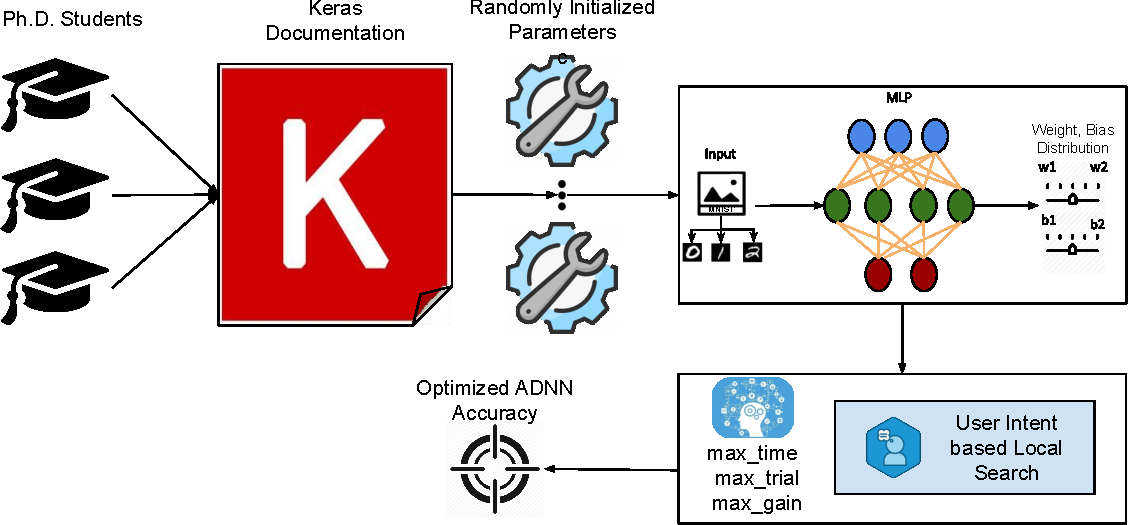
\includegraphics[width=0.95\linewidth]{approach.pdf}
	\centering
	\caption{Overview of the proposed approach}
	\label{fig:flow}
	\vspace{15pt}
\end{figure}
\subsection{Optimized Loss Function}
\subsubsection{5.1.1~~Identifying Randomly Initialized Parameter.}

In this phase, we have to understand the parameters that are subject to the random initialization. For this study, we have already mentioned that our focus has been on the deep learning-based image classifiers. To do so, we have mined the \emph{Keras} \cite{chollet2015keras} documentation to understand the implementation of DNN API. In this process, 3 Ph.D. students have individually gone through the implementation of all the functions. Our goal is two-fold here, 1) Identify the places, where random initialization has taken place that describe the learning-based system, 2) If we can mine the type of distribution from the implementation, then we can understand how the values correspond to that particular parameter has propagated to the output metrics. Our mining technique has identified a class of operation in \emph{Keras} that is responsible for initializing the parameters, called \emph{Initializers.} 
\begin{lstlisting}[language=Python, caption=Example of initialization parameters in Keras]
model.add(Dense(64,
kernel_initializer='random_uniform',
bias_initializer='zeros'))
\end{lstlisting}
The above example of the \emph{initializer} operation in \emph{Keras} can initialize two parameters in the learning process, weight, and bias. The \emph{kernel\_initializer} is responsible for the weight value initialization, while \emph{bias\_initializer} is for bias value corresponds to that particular layer. This serves the purpose of finding the parameters that cause the value of the output to be variant with every execution. 

To identify the distribution of these parameters, we have validated the implementation of the \emph{initializer} class and have found that are a few different distributions that it supports and if not specifically given, which default distribution has been taken care of.
\begin{itemize}
	\item Zeros: This initializes the parameter with 0. While, it may not be an issue for the bias, but if it has been initialized for weight, during the backpropagation, the derivative of the actual and computed value will be 1 for all cases that would make the learning process very hard to compensate the huge loss.
	\item Ones: This initializes the parameter with 1.
	\item Constant: Initializing with a constant is depended on the users' choice of the value.
	\item Normal Distribution: The parameter will be initialized with a normal distribution that takes input as mean ($\mu$) and the standard distribution ($\sigma$) to describe the distribution.
	\item Uniform distribution: This initializes parameter with a uniform distribution where the range of a minimum and maximum value can be specified.
	\item Truncated Normal Distribution: The parameter is initialized with a truncated normal distribution where values greater than 2 standard deviations from mean are omitted. Here, the mean and standard deviation of the random values are used as arguments.
	\item LeCun uniform initializer: This initializes parameter using a uniform distribution where input unit numbers are specified as the limit for drawing samples from it.
	\item Glorot normal initializer: In this initializer, truncated normal distribution using the number of input and output units are used for drawing samples. 
		\begin{lstlisting}[language=Python, caption=Example of Keras's default setup]
	class Dense(Layer):
	def __init__(self, units,
	kernel_initializer='glorot_uniform',
	bias_initializer='zeros',
	....
	**kwargs):\end{lstlisting}
	\item Glorot uniform initializer: This initializes parameter using a uniform distribution where input unit numbers along with the output unit numbers are specified as the limit for drawing samples from it. \\
	We can observe how kernel and bias initializers are initialized from the following example,
	\item LeCun normal initializer: In this initializer, truncated normal distribution using the number of input units are used for drawing samples.
\end{itemize}

%
%\begin{algorithm}
%	\footnotesize
%	\caption{\footnotesize Adaptive Simulated Annealing Based Search.}
%	\label{algo:asa}
%	\begin{algorithmic}[1]
%		\Procedure{asa($model, W_d, B_d$)}{}
%		\State $\delta$=C, $exit\_flag$=False;
%		\For {each $i\in m$}\label{algo1:l3}
%		\State $W_i=0$\label{algo1:l4}
%		\State $B_i=0$\label{algo1:l5}
%		\While{$exit\_flag$=False}\label{algo1:l7}
%		\State $W'=W_i+\delta$
%		\State $B'=B_i+\delta$
%		\If{$W'\in W_d$ and $B'\in B_d$}
%		\State $train(model, W',B')$
%		\State $Obj=L(W_i,B_i)-L(W',B')$
%		\If{$obj\le0$}
%		\State $exit\_flag$=False
%		\Else
%		\State $P=e^{\frac{-obj}{L(W',B')}}$
%		\State $P'=Random()$
%		\If{$P'\le P$}
%		\State  $exit\_flag$=False
%		\EndIf
%		\EndIf
%		\Else
%		\State Go to \ref{algo1:l7}
%		\EndIf
%		\EndWhile
%		\State $W_i=W', B_i=B'$
%		\EndFor\label{algo1:l6}
%		\State \Return $1-L(W,B)$\label{algo2:l12}
%		\EndProcedure\label{algo2:l13}
%	\end{algorithmic} 
%\end{algorithm}


From the \emph{Keras} documentation, we have found that weight and bias parameters are responsible for the change of the output metric in a DNN model. These two parameters are randomly initialized from the user-provided distribution or with the default one. Thus, our goal in this study is to find the value of the bias and weight s.t. the accuracy will be the highest or the loss value will be the least. This is a linear optimization problem, which is solvable in exponential time, but the nearest optimum solution can be achieved in polynomial time. Therefore, we have used an adaptive simulated annealing \cite{ingber2000adaptive} to find the optimized value of the weight and bias combination that leads to better accuracy. 
%In the Algo. \ref{algo:asa}, we have initialized the starting point of the weight and bias to be zero and then we increase the value of the weight and bias initializing value with the step size parameter $\delta$. For each instance, we compute the loss value $L(W, B)$, where $W$ and $B$ represent the initial chosen value of weight and bias. As our goal is to minimize the $L(W, B)$, we run the process until we get a better value. If we get a better result, we validate that the value of the weight and bias do not represent a local minima in the search space, thereupon, we compute a probability value $P$ and a random value in the range $[0,1]$ and similar to the simulated annealing process, we compute the process again the probability is greater than random value. Similarly, we find the value of the weight and bias that provides the near-optimum loss value and with that, we compute the accuracy as $1-L(W, B)$ as in our study, we use the probability as the output metric and $1-loss$ represents the accuracy of the model. In this proposed approach, we start the step size parameter with a constant $C$ that we compute using an empirical evaluation and fix that for a genre of problems.
%\subsubsection{5.1.3~~Ultility}
\subsection{Accountable DNN Accuracy based on User Intent}
In this approach, we have explained how an accountable DNN accuracy can be obtained based on user intent. In terms of user intent, we have introduced max\_time, max\_trial, max\_gain which are described as follows:
\begin{itemize}
	\item \textbf{max\_time} In our approach, we have not restricted to a specific time rather we have provided the user the opportunity to give a certain maximum allowable time until the near-optimal accuracy can be obtained. To emphasize this approach we have empirically run the experiment with two different datasets varying $\delta$ and observe the accuracy based on user given max\_time which has been explained in section \ref{sec:evaluation}. 
	\item \textbf{max\_trial} Similar to the max\_time, we have not restricted the proposed approach to a specific trial as well. Instead, we have also allowed the user to set a certain maximum allowable trial until the near-optimal accuracy can be obtained independent of maximum allowable time. For clarifying the specific scenario of max\_trial, we have conducted an experiment with MNIST, F-MNIST datasets varying $\delta$ and observe the accuracy based on the provided max\_trial which has been explained in section \ref{sec:evaluation}.
	\item \textbf{max\_gain} In addition to max\_time and max\_trial, we have used another user intent i.e., max\_gain. The notion of max\_gain is derived from the difference between actual accuracy and how much accuracy we obtained from our proposed approach. As, we have not confined our approach either to a specific time or a certain trial, we have also made this approach accountable by introducing the concept of user-defined maximum obtained gain in terms of accuracy of a DNN model. Moreover, in section \ref{sec:evaluation}we have shown experimental evaluation about how maximum gain can be achieved using three handmade models of each MNIST, F-MNIST datasets with varying $\delta$ in several trials.          
\end{itemize}
\begin{algorithm}
	\footnotesize
	\begin{algorithmic}[1]
		\State $dataset,batch\_size, learning\_rate, training\_epoch$=user's choice of problem
		\State $count\_hidden=i$
		\State $hidden\_size=[h_1,h_2,...,h_i]$
		\State $init\_weight=[random()_1,...,random()_i]$
		\State $init\_bias=[random()_1,...,random()_i]$
		\State $accuracy\_list=[]$
		\State $trial,gain,time\_diff=0$
		\Procedure{$adnn\_train(max\_time, max\_trial, max\_gain$)}{}
		\State	$(x\_train, y\_train)=dataset.load()$
		\State $current\_time=now()$
		\State $\delta=$ Empirically chosen value(s)
		\For {each $\delta_k$ in $\delta$}
		\State $loss, accuracy\_old=train(init\_weight,init\_bias,$
					\myindent{0.88}$dataset,batch\_size, learning\_rate, training\_epoch)$
		\While {$trial\le max\_trial$ \& $gain\le max\_gain$ \& $time\_diff\le max\_time$}
		\State $init\_weight=init\_weight+\delta_k$
		\State $init\_bias=init\_bias+\delta_k$
		\State $loss, accuracy=train(init\_weight,init\_bias,$
		\myindent{1.28}$dataset,batch\_size, learning\_rate, training\_epoch)$
		\State $accuracy\_list.append(accuracy-accuracy\_old)$
		\State $trial=trial+1$
		\State $time\_diff=now-current\_time$
		\State $gain=max(accuracy\_list)$
		\EndWhile
		\EndFor
		\State \Return $accuracy\_old+gain$
		\EndProcedure
	\end{algorithmic} 
	\caption{\footnotesize ADNN}
	\label{algo:adnn}
\end{algorithm}
In the Algorithm \ref{algo:adnn}, we have utilized the users' intent and have discussed the methodology to perform the searching operation that could be beneficial to increase the accuracy. We have taken the value of the dataset, batch size, learning rate, and epoch parameters from the users as it varies from the choice of the problem and domain. As our proposed approach is currently able to support dense layers, we have taken the number of hidden dense layers present in the model architecture from the users. We have initialized the weight and bias from a random function and the size of the weight and bias is dependent on the size of the hidden layers that users provide. We have denoted the initial starting point of the weight and bias as $init\_weight$ and $init\_bias$ and there will be $i$ number of different weight and bias present, where $i$ denotes the number of allowable hidden layers needed to build the architecture of the model. Then, we have trained the model based on the architecture and the dataset provided. We have not shown the algorithm for the training as we have utilized the MLP implementation of the model building based on \emph{Tensorflow} and in the \emph{Tensorflow} model can be built by providing the weight and bias from the scratch and does not need additional coding to perform a model into its imperative one. Once we have trained the initial model, we have stored the loss and the accuracy of the starting model and have started the searching process. Our searching process is based on the user's intent of the previously defined three parameters i.e., $max\_time$, $max\_trial$, and $max\_gain$. if one of the three conditions does not meet, we have stopped the searching process. During the searching, we have increased the weight and bias value based on the $\delta_k$, where $k$ can be drawn from a set of real numbers that have been chosen based on the empirical evaluation discussed in \S\ref{subsec:result}. We have trained the model with the new sets of weight and bias and store the new accuracy and loss values. We keep on doing the operations until any of the user-provided conditions are met. In the proposed approach, we have defined a metric to measure the increase of the accuracy in each that is defined as \emph{gain}. We have defined \emph{gain} as $gain=accuracy_{T}-accuracy_{M}$, where $accuracy_{T}$ and $accuracy_{M}$ represents as the accuracy of the model after a single trial and accuracy of the model at the start respectively. Once, the algorithm stops, our proposed approach reports the highest gain and the corresponding model to the users.
%\subsection{Assertion of DNN Accuracy}
%This approach includes the validation framework from the learned distribution. We have proposed an assertion mechanism that verify that whether a DNN model can achieve the expected accuracy or not. We propose \emph{ADNN}, a specification language that restricts the learning process from a pair $(f,\nu)$, where $f$ and $\nu$ denotes the learning process and the specification provided by the user. An example of the programming language is depicted as below.
%\begin{lstlisting}[language=Python, caption=Example of specification language]
%@adnn(0.95>accuracy>0.65)
%f(input_image, ....)
%\\Learning operations
%\end{lstlisting}

%\end{itemize}

